\documentclass{beamer} 

\usepackage[utf8]{inputenc}
\usepackage[T1]{fontenc}
\usepackage{graphicx}
\usepackage[serbian]{babel}
\usepackage{multicol}
\usepackage{tikz}
\usetikzlibrary{shapes.geometric, arrows}


\usetheme{Berlin}
\begin{document}


% TikZ blok dijagram stilovi
\tikzstyle{block} = [rectangle, rounded corners, minimum width=3cm, minimum height=1cm, text centered, draw=black, fill=blue!30]
\tikzstyle{arrow} = [thick,->,>=stealth]

\title{VertexVoyage: Distribuirani node2vec algoritam za embedovanje čvorova u realnim mrežama}
\author{Stefan Nožinić \\
Departman za matematiku i informatiku \\
Prirodno-matematički fakultet \\
Univerzitet u Novom Sadu. \\
Tip rada: master rad \\
Mentor: \MakeLowercase{dr} Miloš Savić
}

\frame{
\titlepage
}

\section{Uvod i Motivacija}
\begin{frame}{Uvod}
    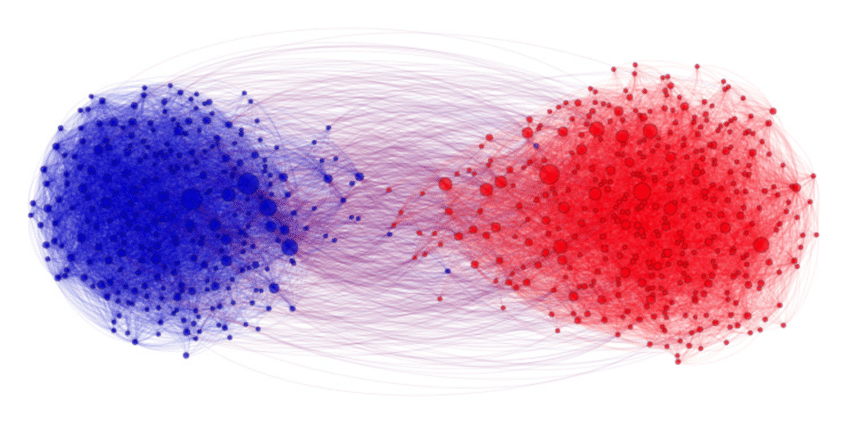
\includegraphics[width=\textwidth]{png/uvod.png}
\end{frame}

\begin{frame}
	\frametitle{Ugrađivanje čvorova}
	Neka je $ G = (V, E) $ graf, tada je ugrađivanje funkcija 

	$$ U : V \to \mathbb{R}^n $$ 

	koja preslikava čvorove grafa u n-dimenzionalni euklidski prostor tako da čvorovi koji su dosta međusobno povezani budu blizu po euklidskom rastojanju
	

\end{frame}

\begin{frame}{node2vec}
	\centering
    \begin{tikzpicture}[node distance=2cm]

    % Blokovi
    \node (walks) [block] {Slučajne šetnje po čvorovima grafa};
    \node (embedding) [block, below of=walks] {Ugrađivanje (Embedding)};

    % Strelice
    \draw [arrow] (walks) -- (embedding);

    \end{tikzpicture}
\end{frame}

\begin{frame}{3 pitanja u radu}
    \centering 
	\begin{tikzpicture}[node distance=2cm]
		\node (q1) [block, text width=8cm, align=center] {Koliko paralelni algoritam ubrzava ceo proces?};
		\node (q2) [block, text width=8cm, align=center, below of=q1] {Kako paralelizacija utiče na kvalitet rekonstrukcije grafa iz ugrađivanja?};		
		\node (q3) [block, text width=8cm, align=center, below of=q2] {Koliko je klasterovanje iz ugrađivanja serijskom implementacijom slično sa klasterovanjem i ugrađivanja paralelnom implementacijom};
	\end{tikzpicture}
\end{frame}


\section{Arhitektura}
\begin{frame}{Arhitektura}
    \centering
    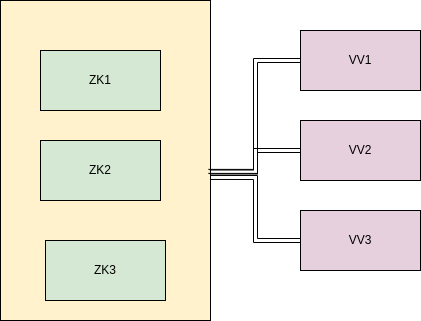
\includegraphics[height=0.8\textheight]{./png/Arhitektura i infrastruktura.drawio.png}
\end{frame}

\section{Generalni Algoritam}
\begin{frame}{Generalni Algoritam}
    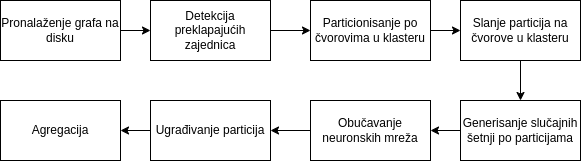
\includegraphics[width=\textwidth]{./png/Blokovski prikaz algoritma.drawio.png}
\end{frame}

\section{Particionisanje}
\begin{frame}{LFM Algoritam}
    \begin{itemize}
        \item Algoritam za detekciju preklapajućih zajednica 
        \item Za svaki čvor koji nije dodeljen zajednici, dodeljuje se nova zajednica 
        \item U zajednicu se dodaju susedni čvorovi čvorova u zajednici takvi da poboljšavaju kvalitet zajednice po funkciji $ f = \frac{k_\text{in}}{(k_\text{out} + k_\text{in})^\alpha} $ 
        \item Nakon dodavanja, čvorovi takvi da njihovo uklanjanje povećava kvalitet zajednice se uklanjaju
        \item Postupak se ponavlja sve dok postoje čvorovi koji nisu dodeljeni nekog zajednici
    \end{itemize}
\end{frame}

\begin{frame}{Modifikacija Algoritma}
    \begin{itemize}
        \item Zbog povećanja brzine, algoritam se modifikuje tako da ne traje sve dok postoje čvorovi koji nisu dodeljeni zajednici
        \item Umesto toga, algoritam se izvršava dok određeni broj čvorova nije dodeljen zajednici
    \end{itemize}
\end{frame}

\begin{frame}{Bin Packing}
    \begin{itemize}
        \item Nakon detekcije zajednica, potrebno je raspodeliti zajednice po čvorovima u klasteru
        \item U ovom radu, koristi se bin packing algoritam
        \item Algoritam raspoređuje zajednice po čvorovima tako da čvorovi u klasteru budu što sličniji po svom opterećenju
        \item Opterećenje čvora K kom su raspoređene zajednice $ S_K $ je $ \sum_{s \in S_K} |s| $
        \item Težine se zatim sortiraju u opadajućem redosledu, počevši od najveće.
        \item Inicijalno, maksimalna veličina (kapacitet) particije je prosečna veličina zajednice 
    \end{itemize}
\end{frame}

\begin{frame}
    \frametitle{Bin packing}
    \begin{itemize}
        \item Algoritam dodeljuje particije zajednicama, počevši od najveće zajednice. Uvek se dodeljuje particija koja je najmanje opterećena
        \item Ukoliko ne postoji particija koja ima potreban kapacitet, kapacitet particija se povećava za prosečnu veličinu zajednice koja još nije dodeljena particiji. 
        \item Ovaj proces se ponavlja dok sve zajednice ne budu raspoređene.
    \end{itemize}
\end{frame}


\section{Gubici strukturnih informacija}
\begin{frame}{Mera gubitka strukturnih informacija}
    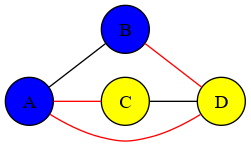
\includegraphics[width=\textwidth]{dot/graf.png}
\end{frame}

\begin{frame}{Mera gubitka strukturnih informacija}
    Neka je $ E_p $ skup svih grana koje sadrže čvorove takve da su oba čvora u particiji $ p $  i neka je $ P $ skup svih particija za graf $ G = (V, E) $

    Tada je mera gubitka strukturnih informacija $ L $ definisana kao

    $$ L = \frac{\sum_{p \in P} |E_p|}{|E|} $$

    Gde je $ |E_p| $ broj grana koje sadrže čvorove iz particije $ p $, a $ |E| $ ukupan broj grana u grafu $ G $
\end{frame}

\section{Node2Vec}
\begin{frame}{Node2Vec}
    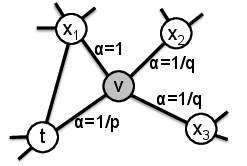
\includegraphics[width=\textwidth]{./png/walk.png}
\end{frame}

\begin{frame}{Word2Vec}
    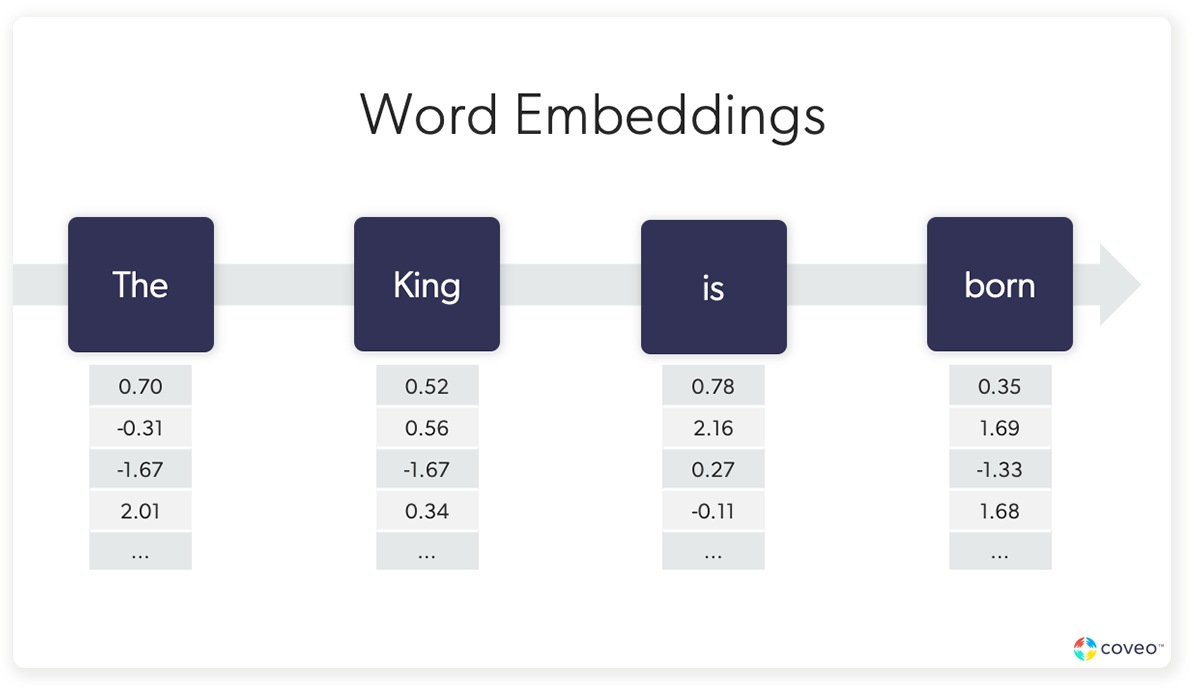
\includegraphics[width=\textwidth]{./png/word2vec.png}
\end{frame}

\section{Rekonstrukcija}
\begin{frame}{Rekonstrukcija}
    $$ \text{recall} = \frac{\sum_{n \in V} \frac{|N(n) \cap N'(n)|}{|N(n)|}}{|V|} $$
    $$ \text{precision} = \frac{\sum_{n \in V} \frac{|N(n) \cap N'(n)|}{|N'(n)|}}{|V'|} $$
    $$ \text{f1} = \frac{2 \cdot \text{precision} \cdot \text{recall}}{\text{precision} + \text{recall}} $$
\end{frame}

\section{KMeans}
\begin{frame}{KMeans Klasterisanje}
    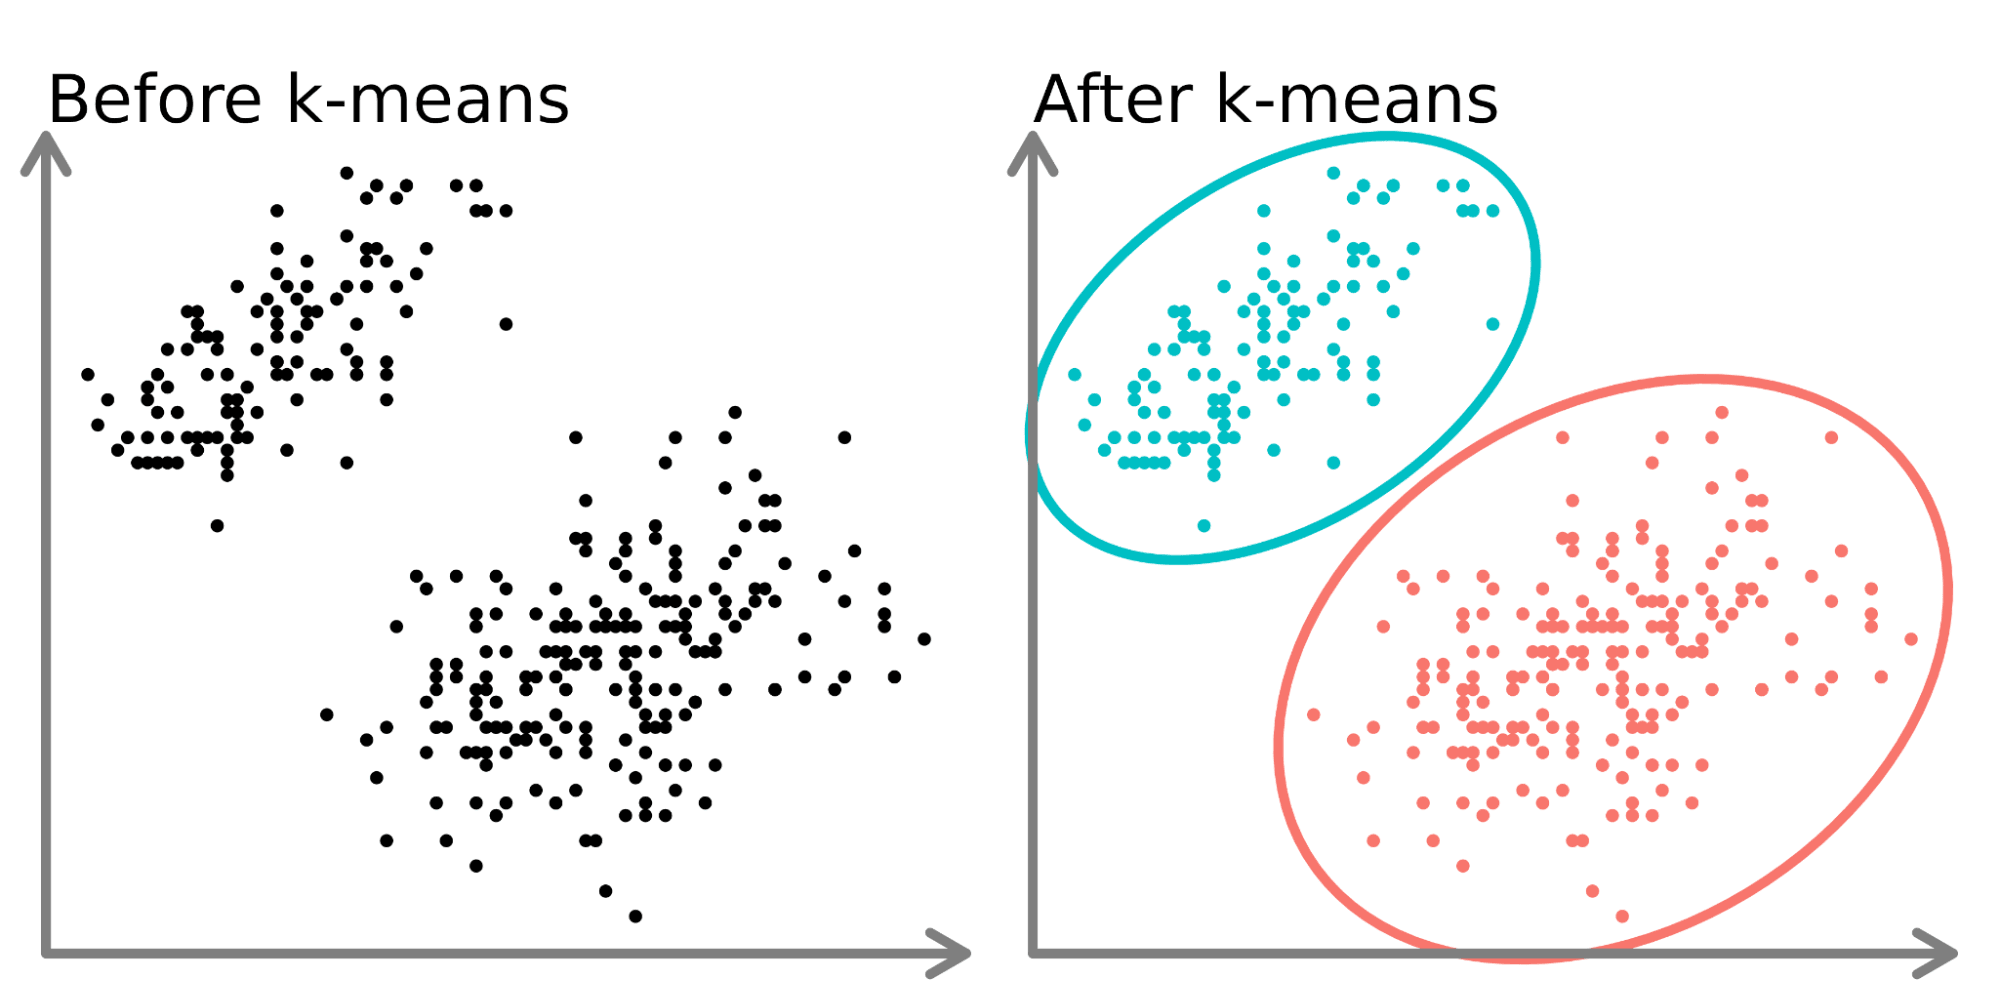
\includegraphics[width=\textwidth]{./png/kmeans.png}
\end{frame}

\section{ARI}
\begin{frame}{Adjusted Rand Index (ARI)}
    \begin{itemize}
        \item Meri sličnost između dve klasterovanja
        \item Vrednost je bliska 0 za slučajno klasterovanje, a 1 za identična klasterovanja
        \item $ \text{ARI} = \frac{\text{RI} - \text{Expected\_RI}}{\text{max(RI)} - \text{Expected\_RI}} $
    \end{itemize}
\end{frame}

\section{Skupovi Podataka}
\begin{frame}{Skupovi Podataka - 1}
    \begin{itemize}
        \item Pregled korišćenih skupova podataka
    \end{itemize}
\end{frame}

\begin{frame}{Skupovi Podataka - 2}
    \begin{itemize}
        \item Detalji o skupovima podataka
    \end{itemize}
\end{frame}

\section{Rezultati}
\begin{frame}{Rezultati - 1}
    \begin{itemize}
        \item Rezultati eksperimenta 1
    \end{itemize}
\end{frame}

\begin{frame}{Rezultati - 2}
    \begin{itemize}
        \item Rezultati eksperimenta 2
    \end{itemize}
\end{frame}

\begin{frame}{Rezultati - 3}
    \begin{itemize}
        \item Rezultati eksperimenta 3
    \end{itemize}
\end{frame}

\begin{frame}{Rezultati - 4}
    \begin{itemize}
        \item Diskusija rezultata
    \end{itemize}
\end{frame}

\begin{frame}{Rezultati - 5}
    \begin{itemize}
        \item Vizuelizacija i poređenje rezultata
    \end{itemize}
\end{frame}

\section{Zaključak}
\begin{frame}{Zaključak}
    \begin{itemize}
        \item Završna razmatranja i budući pravci
    \end{itemize}
\end{frame}


% \begin{frame}
% 	\frametitle{Problem}
% 	% graphics - rendered document and its tree representation 
% 	\begin{columns}
% 		\begin{column}{0.5\textwidth}
% 			\includegraphics[width=\textwidth]{./png/segmented-doc.png}
% 		\end{column}
% 		\begin{column}{0.5\textwidth}
% 			\includegraphics[width=\textwidth]{./png/tree.png}
% 		\end{column}
% 	\end{columns}
% \end{frame}


% \begin{frame}
% 	\frametitle{Reprezentacija celog sistema}
% 	\includegraphics[width=\textwidth]{./png/system.png}
% \end{frame}



% \begin{frame}
% 	\frametitle{Rezultati}
% 	\begin{table}
% 		\begin{tabular}{rllr}
% 		 & Metod kodiranja & Klasifikator & Tačnost (\%)\\
% 		\hline
% 		1 & \texttt{histogram} & RF & 71.792\\
% 		2 & \texttt{img\_attrs} & RF & 72.034\\
% 		3 & \texttt{img\_attrs} & one rule & 63.153\\
% 		4 & \texttt{pixels} & NN & 38.451\\
% 		5 & \texttt{simple} & NN & 42.345\\
% 		6 & \texttt{simple} & RF & 70.422\\
% 		7 & \texttt{simple} & one rule & 63.216\\
% 		\end{tabular}
% 		\caption{Tačnost klasifikatora u odnosu na metode kodiranja}
% 	\end{table}

% \end{frame}

\begin{frame}
	\frametitle{Pitanja}
	\begin{center}
		\huge{?}
	\end{center}
\end{frame}


\end{document}
